\section{Date: 2026-11-02}
\noindent \textbf{Series ID: SMU25781000600000001} 

\noindent This series is titled All Employees: Goods Producing in Springfield, MA-CT (NECTA) and has a frequency of Monthly. The units are Thousands of Persons and the seasonal adjustment is Not Seasonally Adjusted.The observation start date is 1990-01-01 and the observation end date is 2024-12-01.The popularity of this series is 1. \\ 

\noindent \textbf{Series ID: PRGONUPIHCSA} 

\noindent This series is titled Medical Services Expenditures by Provider: Nursing Homes: Proprietary and Government Nursing Homes Price Index and has a frequency of Annual. The units are Index 2017=100 and the seasonal adjustment is Not Seasonally Adjusted.The observation start date is 2000-01-01 and the observation end date is 2021-01-01.The popularity of this series is 1. \\ 

\subsection{Raw Regression}
\noindent Regresses the two series against each other directly. A significant result here can come just as easily from both series sharing a long-run trend as from any real relationship.

\begin{center}
\begin{tabular}{lclc}
\toprule
\textbf{Dep. Variable:}                    & value\_fred\_PRGONUPIHCSA & \textbf{  R-squared:         } &     0.783   \\
\textbf{Model:}                            &            OLS            & \textbf{  Adj. R-squared:    } &     0.772   \\
\textbf{Method:}                           &       Least Squares       & \textbf{  F-statistic:       } &     72.01   \\
\textbf{Date:}                             &      Mon, 02 Nov 2026     & \textbf{  Prob (F-statistic):} &  4.64e-08   \\
\textbf{Time:}                             &          21:06:51         & \textbf{  Log-Likelihood:    } &   -73.979   \\
\textbf{No. Observations:}                 &               22          & \textbf{  AIC:               } &     152.0   \\
\textbf{Df Residuals:}                     &               20          & \textbf{  BIC:               } &     154.1   \\
\textbf{Df Model:}                         &                1          & \textbf{                     } &             \\
\textbf{Covariance Type:}                  &         nonrobust         & \textbf{                     } &             \\
\bottomrule
\end{tabular}
\begin{tabular}{lcccccc}
                                           & \textbf{coef} & \textbf{std err} & \textbf{t} & \textbf{P$> |$t$|$} & \textbf{[0.025} & \textbf{0.975]}  \\
\midrule
\textbf{const}                             &     186.2043  &       11.787     &    15.797  &         0.000        &      161.616    &      210.793     \\
\textbf{value\_fred\_SMU25781000600000001} &      -2.2652  &        0.267     &    -8.486  &         0.000        &       -2.822    &       -1.708     \\
\bottomrule
\end{tabular}
\begin{tabular}{lclc}
\textbf{Omnibus:}       &  5.822 & \textbf{  Durbin-Watson:     } &    0.251  \\
\textbf{Prob(Omnibus):} &  0.054 & \textbf{  Jarque-Bera (JB):  } &    4.103  \\
\textbf{Skew:}          &  1.043 & \textbf{  Prob(JB):          } &    0.129  \\
\textbf{Kurtosis:}      &  3.353 & \textbf{  Cond. No.          } &     333.  \\
\bottomrule
\end{tabular}
%\caption{OLS Regression Results}
\end{center}

Notes: \newline
 [1] Standard Errors assume that the covariance matrix of the errors is correctly specified.

\begin{figure}
\centering
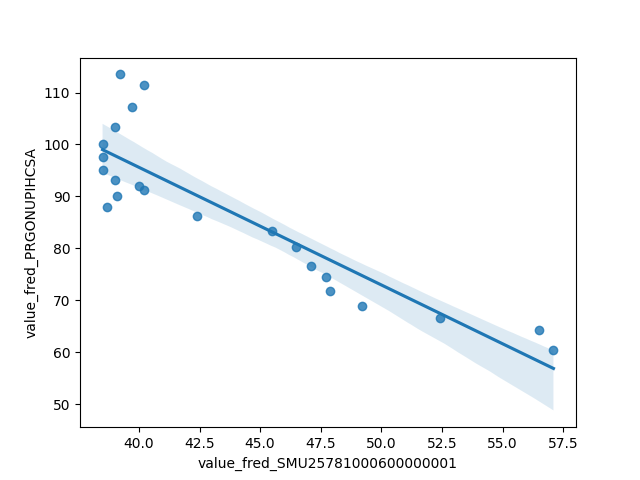
\includegraphics[scale = 0.9]{plots/plot_2026-11-02.png}
\caption{Raw Regression Plot for 2026-11-02}
\end{figure}
\newpage
\subsection{Detrended Regression}
\noindent Regresses the residuals of each series after removing its own linear time trend, so a shared trend can no longer drive the result on its own. A relationship that stays significant here is better evidence of a genuine link between the two series.

\begin{center}
\begin{tabular}{lclc}
\toprule
\textbf{Dep. Variable:}                               & value\_fred\_PRGONUPIHCSA\_detrended & \textbf{  R-squared:         } &     0.021   \\
\textbf{Model:}                                       &                 OLS                  & \textbf{  Adj. R-squared:    } &    -0.028   \\
\textbf{Method:}                                      &            Least Squares             & \textbf{  F-statistic:       } &    0.4223   \\
\textbf{Date:}                                        &           Mon, 02 Nov 2026           & \textbf{  Prob (F-statistic):} &    0.523    \\
\textbf{Time:}                                        &               21:06:51               & \textbf{  Log-Likelihood:    } &   -42.096   \\
\textbf{No. Observations:}                            &                    22                & \textbf{  AIC:               } &     88.19   \\
\textbf{Df Residuals:}                                &                    20                & \textbf{  BIC:               } &     90.37   \\
\textbf{Df Model:}                                    &                     1                & \textbf{                     } &             \\
\textbf{Covariance Type:}                             &              nonrobust               & \textbf{                     } &             \\
\bottomrule
\end{tabular}
\begin{tabular}{lcccccc}
                                                      & \textbf{coef} & \textbf{std err} & \textbf{t} & \textbf{P$> |$t$|$} & \textbf{[0.025} & \textbf{0.975]}  \\
\midrule
\textbf{const}                                        &    4.027e-13  &        0.367     &   1.1e-12  &         1.000        &       -0.765    &        0.765     \\
\textbf{value\_fred\_SMU25781000600000001\_detrended} &      -0.0866  &        0.133     &    -0.650  &         0.523        &       -0.365    &        0.191     \\
\bottomrule
\end{tabular}
\begin{tabular}{lclc}
\textbf{Omnibus:}       &  2.262 & \textbf{  Durbin-Watson:     } &    0.331  \\
\textbf{Prob(Omnibus):} &  0.323 & \textbf{  Jarque-Bera (JB):  } &    1.135  \\
\textbf{Skew:}          & -0.097 & \textbf{  Prob(JB):          } &    0.567  \\
\textbf{Kurtosis:}      &  1.904 & \textbf{  Cond. No.          } &     2.75  \\
\bottomrule
\end{tabular}
%\caption{OLS Regression Results}
\end{center}

Notes: \newline
 [1] Standard Errors assume that the covariance matrix of the errors is correctly specified.

\begin{figure}
\centering
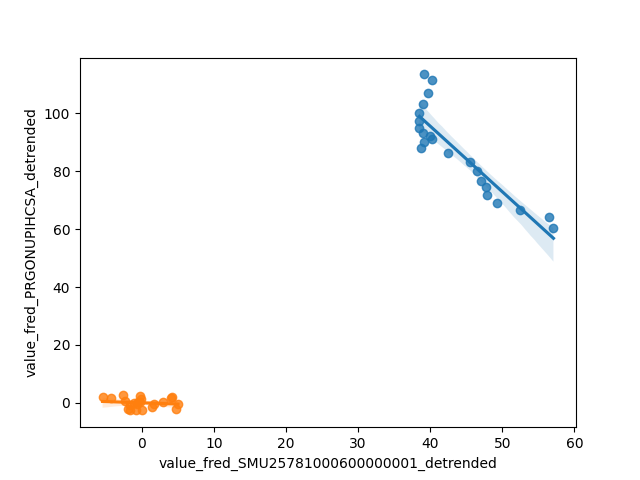
\includegraphics[scale = 0.9]{plots/plot_2026-11-02_detrended.png}
\caption{Detrended Regression Plot for 2026-11-02}
\end{figure}
\newpage
